
\documentclass[paper=a4,DIV15,oneside,lefteqn,american]{scrartcl}
\pdfoutput=1

\usepackage[american,german]{babel} 
\usepackage[margin=1.2in]{geometry}

\usepackage[T1]{fontenc}
\usepackage[utf8]{inputenc}

\usepackage{hyperref}
\usepackage[pdftex]{graphicx}
\usepackage{xspace}
\usepackage{textcomp}
\usepackage{framed}

\usepackage[draft,inline,nomargin]{fixme}

\usepackage{verbatim}

\usepackage{amsmath}
\usepackage{amssymb}
\usepackage{amsthm}
\usepackage{txfonts}
\usepackage{mathtools}

\addtolength{\parskip}{0.5\baselineskip}
\parindent=0cm



\newcommand{\VV}{Verification \& Validation\xspace}
\newcommand{\vv}{verification \& validation\xspace}

\def\CC{{C\nolinebreak[4]\hspace{-.05em}\raisebox{.4ex}{\tiny\bf ++}}}

\newcommand{\bitwalker}{\mbox{\texttt{Bitwalker}}\xspace}

\newcommand{\poke}{\mbox{\texttt{Bitwalker\_Poke}}\xspace}
\newcommand{\peek}{\mbox{\texttt{Bitwalker\_Peek}}\xspace}
\newcommand{\acsl}{\mbox{\textsf{ACSL}}\xspace}
\newcommand{\isoc}{\mbox{\textsf{C}}\xspace}
\newcommand{\framac}{\mbox{\textsf{Frama-C}}\xspace}
\newcommand{\framacwp}{\mbox{\textsf{Frama-C\slash WP}}\xspace}
\newcommand{\why}{\mbox{\textsf{Why}}\xspace}
\newcommand{\wpframac}{\mbox{\textsf{WP}}\xspace}
\newcommand{\altergo}{\mbox{\textsf{Alt-Ergo}}\xspace}
\newcommand{\qed}{\mbox{\textsf{Qed}}\xspace}
\newcommand{\cvc}{\mbox{\textsf{CVC4}}\xspace}
\newcommand{\z}{\mbox{\textsf{Z3}}\xspace}
\newcommand{\coq}{\mbox{\textsf{Coq}}\xspace}
\newcommand{\cealist}{\mbox{\textsf{CEA LIST}}\xspace}

\newcommand{\inl}[1]{\lstinline[style=inline]{#1}}


%Defining C-Code Environment

\usepackage{courier} 
\usepackage{listings}
\usepackage{color} 

% fix bug with listing under texlive-2014
% see https://lists.debian.org/debian-tex-maint/2014/06/msg00209.html

\makeatletter
\renewcommand\lstinline[1][]{%
  \leavevmode\bgroup % \hbox\bgroup --> \bgroup
  \def\lst@boxpos{b}%
  \lsthk@PreSet\lstset{flexiblecolumns,#1}%
  \lsthk@TextStyle
  \ifnum\iffalse{\fi`}=\z@\fi
  \@ifnextchar\bgroup{%
  \ifnum`{=\z@}\fi%
  \afterassignment\lst@InlineG \let\@let@token}{%
  \ifnum`{=\z@}\fi\lstinline@}}
\makeatother


%\definecolor{darkred}		{rgb}{0.60,0.00,0.00}
\definecolor{coACSLBehavior}	{rgb}{0.30,0.00,0.00}
\definecolor{coASCL}		{rgb}{0.00,0.10,0.00}
\definecolor{coASCLKeyword}	{rgb}{0.00,0.10,0.10}
\definecolor{darkgreen}		{rgb}{0.00,0.40,0.00}
%\definecolor{red}		{rgb}{0.98,0.00,0.00}
\definecolor{darkblue}		{rgb}{0.00,0.00,0.60}
%\definecolor{lightblue}		{rgb}{0.60,0.80,1.00}
%\definecolor{lightred}		{rgb}{1.00,0.60,0.60}
\definecolor{coCKeyword}	{rgb}{0.00,0.00,0.60}

\lstdefinestyle{acsl-block}
{	emph=[1]{assert, assumes, assigns, axiom, axiomatic, decreases, ensures,
                 ghost, invariant, lemma, logic, loop, predicate,
		 reads, requires, variant},
	emphstyle=[1]{\bfseries\color{coASCLKeyword}},
	emph=[2]{behavior, behaviors, complete, disjoint, for:},
	emphstyle=[2]{\bfseries\color{coACSLBehavior}},
	emph=[3]{typedef, int, char, integer, real, bool, size_type, value_type, uint8_t,  uint64_t},
	emphstyle=[3]{\bfseries\color{coCKeyword}},
	escapeinside={//`}{`//},
	morecomment=*[l][\color{coASCL}]{//@},
	morecomment=*[s][\color{coASCL}]{/*@}{*/},
	moredelim=*[is][\bfseries]{|*}{*|},
	%emphstyle=[3]{\ttfamily}
	}

\lstdefinestyle{func-decl}
{	emph=[1]{assert, assumes, assigns, axiom, axiomatic, decreases, ensures,
                 ghost, invariant, lemma, logic, loop, predicate,
		 reads, requires, variant},
	emphstyle=[1]{\bfseries\color{coASCLKeyword}},
	emph=[2]{behavior, behaviors, complete, disjoint, for:},
	emphstyle=[2]{\bfseries\color{coACSLBehavior}},
	emph=[3]{integer, real, size_type, value_type},
	emphstyle=[3]{\bfseries\color{coCKeyword}},
	escapeinside={//`}{`//},
	morecomment=*[l][\color{coASCL}]{//@},
	morecomment=*[s][\color{coASCL}]{/*@}{*/},
	moredelim=*[is][\bfseries]{|*}{*|},
    frame=none,
    numbers=none
	%emphstyle=[3]{\ttfamily}
	}

\lstdefinestyle{acsl-inline}
{	emph=[1]{assert,assigns, assumes, axiom, axiomatic, decreases, ensures, ghost, invariant, lemma, logic, loop,
             predicate, reads, requires, return, variant },
	emphstyle=[1]{\bfseries\color{coASCLKeyword}},
	emph=[2]{behavior, behaviors, complete, disjoint, for:},
	emphstyle=[2]{\bfseries\color{coACSLBehavior}},
	emph=[3]{typedef, int, char, integer, real, bool, size_type, value_type, uint8_t,  uint64_t},
	emphstyle=[3]{\bfseries\color{coCKeyword}},
	morecomment=*[l][\color{coASCL}]{//@},
	morecomment=*[s][\color{coASCL}]{/*@}{*/},
	moredelim=*[is][\bfseries]{|*}{*|}
}

\lstdefinestyle{inline}
{      % basicstyle = \ttfamily\small\color{coASCL},
	keywordstyle = \ttfamily\small\color{coASCL},
	stringstyle=\color{coASCL},
	style=acsl-inline,
	breaklines= false
}

\lstset{%
  language=C++,
  defaultdialect=ansi,
  basicstyle=\small\ttfamily,
  commentstyle=\small\color{darkgreen},
  keywordstyle=\small\bfseries\color{darkblue},
  stringstyle=\small\color{darkgreen},
  tabsize = 2,
  showspaces=false,
  showtabs=false,
  columns=fixed,  
  frame=none,  
  breaklines=true,
  showstringspaces=false,
  xleftmargin=0.2cm,
  %rangeprefix=//label, % to specify a certain range from a file
  %rangesuffix=;, % to be shown
  %includerangemarker=false,
	numbers=none
}


\title{Informal Specification of \bitwalker}
\author{Jens Gerlach\\
        {\small Fraunhofer FOKUS, Berlin, Germany}
       }
\date{}

\begin{document}
\selectlanguage{american}
\maketitle
\thispagestyle{empty}

\begin{abstract}
Starting from the original high-level description of the \bitwalker
software this document provides a more detailed, but still informal,
specification.
This specification attempts to be precise to the extend that
\begin{enumerate}
\item
testers are able to write unit tests for \bitwalker without the need to
look at its implementation

\item
it can serve as a base for a \emph{formal} specification in the
\acsl specification language of \framac.
\end{enumerate}
\end{abstract}


\tableofcontents
\clearpage
\listoffixmes

%-----------------------------------------------------------------------
\section*{Introduction}
%-----------------------------------------------------------------------

\subsection*{Objectives}

\emph{Verification} is the activity to ascertain that a particular
step in the development has achieved its goals, i.e., that its result
correctly refines or implements its input, which may be a higher-level
design or a specification. \emph{Validation} is about making sure that
the end result of the development meets its initial specification,
that is, the requirements of the user. The term validation is also
used when a design artifact is checked against requirements from
previous steps. Verification and/or validation is required for most
development artifacts.  What exactly has to be checked depends on the
set of items produced in the development process, their role and their
nature.  As the EVC software contributes to several safety-critical
functions of the ETCS onboard unit, the specific requirements
concerning the safety aspects of the standards EN~50128 and EN~50129
have to be respected throughout.

A main obligation of this work package is the verification or
validation of development artifacts produced by WP~3. This work will
concentrate on the functional and safety aspect. Besides \vv,
the work package shall also establish a coherent and comprehensive
chain of methods and tools for V\&V in cooperation with WP~7. Specific
challenges in this respect arise from the wish to use models
extensively in the development process, which means that more common
approaches have to be improved or substituted to fit a
model-based development style, and from the requirement of
using open-source tools, or even trying to realize the EVC software as
an \emph{open proof} item.

In pursuing these goals, the work package generates feedback
concerning the adequacy, correctness and safety of development
artifacts for WP~3, and the usefulness of tools and methods for WP~7.  

\subsection*{Organisation of the Work package}

The work packages consists of five tasks. The first task defines the
\vv strategy and formulates the initial \vv plan. This plan defines the
\vv activities to be done in openETCS and proposes the means to
perform them. In later stages of the project the plan will be extended
and revised to reflect the findings made while applying methods and
tools to the artifacts at hand.

Both model and code of the EVC software are subjected to \vv as they
are produced by WP~3, and the tools and methods proposed in the \vv
plan as well as newly developed or improved tools from WP~7 are applied
and evaluated in the process. Findings from these steps are
iteratively fed back to the respective work package and used to refine
the \vv plan.

A dedicated activity studies the safety aspect of \vv. It takes into
consideration what the standards (mainly EN~50128 and EN~50129) mandate
and defines how these requirements can be met by the combination of
life cycle, methods and tools.

An internal assessment will simulate a real Assessor's task doing a 
Software Development assessment of the project impacting Working Packages 
1, 2, 3, 4, 5, 6 and 7.

The phases defining the \vv process is divided into the design phase and 
the application phase. The \emph{design phase} covers the time before the 
release of the artifacts which are to be evaluated. In this phase the 
findings of the last application phase are taken into account to improve 
\vv.
The \emph{application phase} covers the time after the release of the 
artifacts to be evaluated until the \vv report is written. For this phase 
the artifacts to be evaluated are frozen to a fixed release date.  

%-----------------------------------------------------------------------
\subsection*{Techniques for \VV}
%-----------------------------------------------------------------------

\VV techniques can be roughly classified into \emph{dynamic} and
\emph{static} techniques.  The most common dynamic \vv techniques are
various forms of \emph{testing}, which execute the code or the
model. They are classified by their object or their purpose. These
include:
\begin{itemize}
\item Unit testing
\item Integration testing
\item Acceptance test
\item Software-in-the-Loop
\item Model-in-the-Loop
\item Model-based testing
\item Monitoring
\item Coverage analysis
\end{itemize}
A related dynamic activity is \emph{animation}, which may play a role
in analyzing an executable model.

Static \vv techniques---not executing model or code---include:
\begin{itemize}
\item Checking of coding guidelines
\item Review
\item Walkthrough
\item Formal methods
\begin{itemize}
\item Model checking
\item Deductive verification (theorem proving)
\item Abstract interpretation
\end{itemize}
\end{itemize}

%\begin{figure}[h]
%\centering
%\input{sections/openETCSOpenProofsDevelopmentProcess.pdf_tex}
%\caption{openETCS open proofs concept}
%\end{figure}

\todo{description on V\&V classification non formal-> formal -> formal
  -> code \& description}

\subsection*{Coping with a Model-Based Development Style}

Models appear at different stages of the development. An important
artifact of openETCS is a semi-formal model of the requirements. 
Depending on the modelling framework, the modelling language and
formalization of the system requirements a
concept has to be defined how the consistency and coherence of the
model as well as the coverage of system requirements will be
transparently verified. For this task, static verification techniques
will very likely offer the best approach.

To verify that the model correctly captures the ETCS system
requirement specification (Subset-026 et. al.), also dynamic techniques
like animation might be useful. And finally, it may be helpful to also
validate the model against the user requirements.

For later development stages, correct refinement or implementation of
the model will have to be established. Again, techniques to be applied
depend heavily on the nature of the model(s) and the process of how
the code is derived. Model-based testing, i.e., deriving test cases
from a model to ascertain that an executable behaves consistent to a
model, is a technique to be used. Alternatively, if code is generated
automatically from a model, other means like tools checking the
correctness of a generation procedure (or its outcome on a
case-by-case basis) may be chosen.

An important issue to be kept in mind is the suitability of models
and tools for a safety-critical development. Modelling languages that
lack a formal semantics or the expressive power to capture system
aspects essential for safety considerations are of limited
usefulness. And tools need to be qualifiable according to their role.  
For instance, a code generator needs to be verified or qualified or it
must be accompanied by some tool checking the correctness of the
generation step. Otherwise, the resulting code will have to verified
similar as manually written code.





\chapter{Basic concepts}
\label{sec:basic}

\begin{itemize}
\item
A \emph{bit stream} is an array containing elements of type \verb"uint8_t".

A bit stream of length $n$ contains $8n$ bits.

\item
A bit stream is \emph{valid} if the array is valid.

\item 
A bit stream can be indexed both by its array indices
and its \emph{bit indices}.

Figure~\ref{fig:bitstream-indices} shows the difference between 
array indices and bit indices in a bit stream.
The two bit indices, 0~and~14,
mark bit positions in the first and second array element, respectively.

\begin{figure}[hbt]
\begin{center}
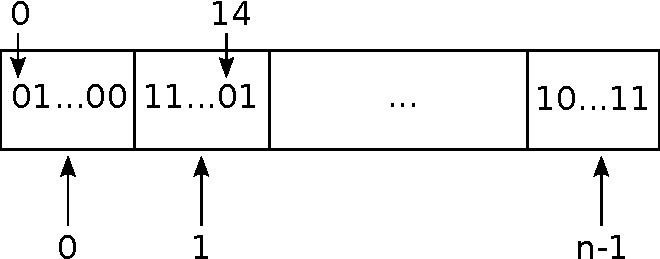
\includegraphics[width=0.40\textwidth]{figures/array_as_stream.pdf}
\caption{\label{fig:bitstream-indices} Array indices and bit indices in a bit stream}
\end{center}
\end{figure}

\item 
The C~programming language neither provides a type \emph{bit}
nor does it support random access to the bits of a bit stream.
In order to access the $i$-th bit of a bit sequence one typically
has to first access the byte with index $j = i/8$ and then access the 
bit $k = i \pmod{8}$ within this byte.
Note that in Figure~\ref{fig:bitstream-indices} 
bytes and bits are indexed in increasing order from the \emph{left}.
On the byte level, however, bits are often indexed from the \emph{right}.
For example, to access the $k$-th bit of a byte \inl{a} one can
shift this bit to the right by $7-k$ and extracts then the now
rightmost bit by performing a bit-wise \emph{and} with the value~1
%
\begin{verbatim}
   (a >> (7-k)) & 1
\end{verbatim}

\item
A \emph{bit sequence} is a consecutive sequence of bits within a bit stream
as represented in Figure~\ref{fig:bitsequence}.
\begin{figure}[hbt]
\begin{center}
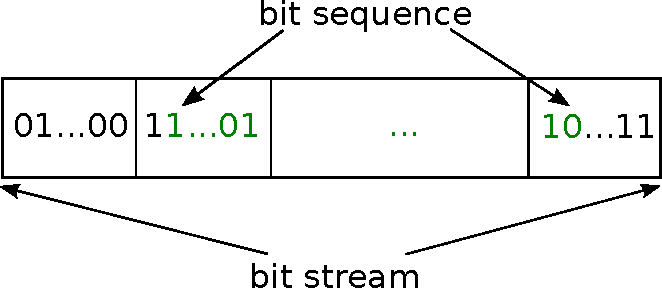
\includegraphics[width=0.40\textwidth]{figures/bit_sequence.pdf}
\caption{\label{fig:bitsequence} A bit sequence within a bit stream}
\end{center}
\end{figure}

A bit sequence is given by the position of its first bit (a bit index in the bit stream)
and its \emph{length}, that is, the number of bits it contains.

\item

A bit sequence that starts at bit index $p$ and that consists of
length $l \geq 0$ is refered to \emph{valid} (with respect to a bit stream of length $n$)
if the following conditions are satisfied
\begin{align*}
  0 &\leq p < 8n \\
  0 &\leq p + l \leq 8n
\end{align*}

Not that only the bits with indices $p \leq i < p + l$ are to be accessed
but not the bit with index~$p+l$.

\end{itemize}

We assume that the C-types \inl{unsigned int} and \inl{int}, which
are used in the implementation to represent indices, counting and error codes,
have a width of~32~bits.
We point this out here because we conducted the verification on a platform with
these characteristics.

As an aside, MISRA-C discourages the use of ``generic'' integer types
such as \inl{int} and \inl{unsigned int} and recommends the use of integer types whose names
contain the exact width.




\chapter{The public interface of \bitwalker}

\section{The structure \bitwalkertype}


In this section we specify the object \locals.  The signature of the object reads:

\begin{lstlisting}[style=acsl-block]
   typedef struct
   {
       uint8_t       *Bitstream;
       unsigned int  Length;
       unsigned int  CurrentBitposition;
   } T_Bitwalker_Incremental_Locals;
\end{lstlisting}


\paragraph{Description}

\begin{itemize}

   \item \inl{Bitstream} is  the start address of a valid bit stream.
   \item \inl{Length} is the length of the bit stream, that starts at \inl{Bitstream}.
   \item \inl{CurrentBitposition} is a valid bit index in the bit stream given by \inl{Bitstream} and \inl{Length}

\end{itemize}
\fxfatal{\inl{Length} should be named \inl{Size}, because it characterizes the Length of \inl{Bitstream} and not of a sequence.}

\clearpage

\section{Informal Specification of \inl{Bitwalker_IncrementalWalker_Init}}

In this section we specify the function \init.  The function  initializes object of the type \locals.
The function signature reads:


\begin{lstlisting}[style=acsl-block]
void Bitwalker_IncrementalWalker_Init(
        T_Bitwalker_Incremental_Locals *Locals,
        uint8_t Bitstream[],
        unsigned int Size,
        unsigned int FirstBitposition);
\end{lstlisting}


\paragraph{Arguments}
\begin{itemize}
   \item  \inl{Locals} is a dereferenceable pointer.
   \item \inl{Bitstream} is  the start address of a valid bit stream.
   \item \inl{Size} is the length of the bit stream, that starts at \inl{Bitstream}.
   \item \inl{FirstBitposition} is a valid bit index in the bit stream given by \inl{Bitstream} and \inl{Size}
\end{itemize}

\paragraph{Preconditions}
\begin{itemize}
    \item  \inl{Locals} must me dereferenceable.
\end{itemize}

\paragraph{Description}\hfill\\\hfill
The function \init assigns:
\begin{itemize}
    \item \inl{Bitstream}  to \inl{Locals->Bitstream}.
    \item \inl{Size} to \inl{Locals->Length}
    \item \inl{FirstBitposition} to \inl{Locals->CurrentBitposition}
\end{itemize}
\fxfatal{\inl{Size} is length of the \inl{Bitstream} not of a \inl{sequence}, So \inl{Locals->Length} should be named \inl{Locals.Size}}

\clearpage

\section{Informal Specification of \inl{Bitwalker_IncrementalWalker_Peek_Next}}

In this section we examine the function \peeknext in the same manner as we did it for \init.
The function \peeknext reads a sequence from a bit stream  and sets the index of the bit stream  to the first position behind .
stream. Its function signature reads as follows:


\begin{lstlisting}[style=acsl-block]
uint64_t Bitwalker_IncrementalWalker_Peek_Next (
    T_Bitwalker_Incremental_Locals *Locals,
    unsigned int Length);
\end{lstlisting}


\paragraph{Arguments}
\begin{itemize}
   \item  \inl{Locals} is a dereferenceable pointer.
   \item \inl{Length} is the Length of the sequence.
\end{itemize}

\paragraph{Preconditions}
\begin{itemize}
    \item  \inl{Locals} must me dereferenceable.
    \item \inl{Length} $\leq$ \inl{64} and
    \item \inl{Locals.CurrentBitposition} $\leq $ \inl{UINT_MAX} $-$ \inl{Length}
\end{itemize}

\paragraph{Description}

\peeknext reads a sequence from a bit stream and  returns it as $64$ bit integer. If the bit sequence is not valid the function shall return \inl{0}. Furthermore  it sets \inl{Locals.CurrentBitposition} to the first position behind the sequence that was read. All other components of \inl{Locals} are not altered.




\clearpage

\section{Informal Specification of \inl{Bitwalker_IncrementalWalker_Peek_Finish}}

\begin{lstlisting}[style=acsl-block]
int Bitwalker_IncrementalWalker_Peek_Finish (T_Bitwalker_Incremental_Locals *Locals);
\end{lstlisting}

\paragraph{Arguments}

\begin{itemize}
    \item  \inl{Locals} holds a bit stream, the start position and the length of the bit stream.
\end{itemize}

\paragraph{Preconditions}
\begin{itemize}
    \item  \inl{Locals} is a valid record.
    \item \inl{Locals.CurrentBitposition} $\leq $ \inl{UINT_MAX}.
\end{itemize}

\paragraph{Description}

\peekfinish  returns the current bit position of the bit stream that is hold by \inl{Locals}.

\fxfatal{Should the return value be an unsigned type?}

\clearpage

\section{Informal Specification of \inl{Bitwalker_IncrementalWalker_Poke_Next}}
\begin{lstlisting}[style=acsl-block]
int		 Bitwalker_IncrementalWalker_Poke_Next(T_Bitwalker_Incremental_Locals *Locals, unsigned int Length, uint64_t Value);
\end{lstlisting}

\paragraph{Arguments}

\begin{itemize}
    \item  \inl{Locals} holds a bit stream, the start position of the sequence within the bit stream.
   \item \inl{Length} is the Length of the sequence.
   \item \inl{Value} is the integer which shall be converted into a bit sequence
\end{itemize}

\paragraph{Preconditions}
\begin{itemize}
    \item  \inl{Locals} is a valid record.
    \item \inl{Locals.CurrentBitposition} + \inl{Length} is less than \inl{UINT_MAX}
\end{itemize}

\paragraph{Description}

We specify \pokenext as follows:
The function \poke converts a 64-bit unsigned integer to a bit sequence and 
writes it into a bit stream.

For $0 \leq x$ exists a shortest sequence of~0 and~1
$(b_0, b_1,\ldots,b_{n - 1})$
such that
\begin{align}
    \sum_{i=0}^{n-1} b_i \cdot 2^{(n - 1) - i} = x.
\end{align}

The function \pokenext tries to store the sequence $(b_0, b_1,\ldots,b_{n - 1})$
in the bit sequence of \inl{Length} bits that starts
at bit index \inl{Locals.CurrentBitposition}.

The return value depends on  the following cases:
\begin{itemize}
    \item  If the bit sequence is not valid \peeknext  returns $-1$.
    \item  If the bit sequence is valid, then there are two cases:
\begin{itemize}
\item
If $x$ is greater or equal than $2^\mathtt{Length}$, then~$x$
cannot be represented as bit sequence $(b_0, b_1,\ldots,b_{\mathtt{Length} - 1})$.
\pokenext returns then~$-2$.

\item
If $x$ is less the $2^{\mathtt{Length}}$, then  the sequence
$(\overbrace{0,\ldots,0}^{\mathtt{Length}-n},b_0, b_1,\ldots,b_{n - 1})$
is stored in the bit stream starting at \inl{Locals.CurrentBitposition}.
The return value of \pokenext is 0.

\end{itemize}
\end{itemize}

Regardless of whether the poke was successful \pokenext sets the value  \inl{Locals.CurrentBitposition} to the first position behind the sequence that it tired to poke.
 All other components of the record \inl{Locals} remain unaltered.


\clearpage

\section{Informal Specification of \inl{Bitwalker_IncrementalWalker_Poke_Finish}}

\begin{lstlisting}[style=acsl-block]
int		 Bitwalker_IncrementalWalker_Poke_Finish (T_Bitwalker_Incremental_Locals *Locals);
\end{lstlisting}

\paragraph{Arguments}
\begin{itemize}
    \item  \inl{Locals} holds a bit stream, the start position and the length of the bit stream.
\end{itemize}

\paragraph{Preconditions}
\begin{itemize}
    \item  \inl{Locals} is a valid record.
    \item \inl{Locals.CurrentBitposition} $\leq $ \inl{UINT_MAX}.
\end{itemize}

\paragraph{Description}

\peekfinish  returns the current bit position of the bit stream that is hold by \inl{Locals}.




\section{Specification of \peek and \poke}

\subsection{Informal specification of \peek}
\label{sec:informal-peek}

Now we specify \peek with the introduced auxiliary concepts.
The function \peek reads a bit sequence from a bit stream
and converts it to an integer.

Its function signature reads as follows:

\begin{lstlisting}[style=acsl-block]
uint64_t  Bitwalker_Peek(unsigned int Startposition, 
                         unsigned int Length,
                         uint8_t Bitstream[],
                         unsigned int BitstreamSizeInBytes);
\end{lstlisting}

\paragraph{Arguments}
The arguments of \peek have the following purpose:
\begin{itemize}
    \item \inl{Startposition} is the bit index in the bit stream 
    where the bit sequence starts.
    \item \inl{Length} is the length of the bit sequence.
    \item \inl{Bitstream} is the array which provides the bit stream.
    \item \inl{BitstreamSizeInBytes} is the length of the array 
    containing the bit stream. 
\end{itemize}

\paragraph{Preconditions}
The following preconditions shall hold for the function arguments.
Note that additional constraints are implicitly expressed by the use
of \emph{unsigned} integer types.

\begin{itemize}
\item \inl{Bitstream} is a valid array of length \inl{BitstreamSizeInBytes}

\item \inl{Length} $\leq$ \inl{64} and

\item \inl{Startposition} $\leq$ \inl{UINT_MAX} - \inl{Length}.
      This condition expresses that no arithmetic overflows shall occur
      when evaluating \inl{Startposition + Length}.
\end{itemize}

\paragraph{Description}
As mentioned, the function \peek reads a bit sequence from a bit stream
and converts it to a 64-bit unsigned integer.

For a bit sequence $(b_0, b_1,\ldots,b_{n - 1})$ the function \peek returns the sum
\begin{align}
\label{eq:peek-result}
    \sum_{i=0}^{n-1} b_i \cdot 2^{(n - 1) - i} 
\end{align}

Note that is a higher-level description than what is done in the source code.
There is, in our opinion, not much point to reflect all of the low-level bit operations
into the specification if a clearer description is at hand.

If the bit sequence is not valid, then \peek shall return~0.
We were wondering why the implementation maps an illegal input to a legitimate output.
The code providers argued along the lines that this error condition was not
considered important enough to be properly reported.
One can interpret this design decision as an attempt to increase the
robustness of the function against illegal values.
In general, we recommend to explicitly describe all error conditions
and to devise a consistent error detection and error recovery strategy.


\subsection{Informal specification of \poke}
\label{sec:informal-poke}

In this section we examine the function \poke
in the same manner as we did it for \peek.

The function \poke converts an integer to a bit sequence and writes it
into a bit stream.
Its function signature reads as follows:
\begin{lstlisting}[style = acsl-block]
int      Bitwalker_Poke(unsigned int Startposition,
                        unsigned int Length,
                        uint8_t Bitstream[],
                        unsigned int BitstreamSizeInBytes,
                        uint64_t Value);
\end{lstlisting}


\paragraph{Arguments}
The arguments have the following purpose:

\begin{itemize}
    \item \inl{Startposition} is the bit index in the bit stream 
    where the bit sequence starts.
    \item \inl{Length} is the length of the bit sequence.
    \item \inl{Bitstream} is the array which provides the bit stream.
    \item \inl{BitstreamSizeInBytes} is the length of the array 
    containing the bit stream. 
    \item \inl{Value} is the integer which shall be converted into a bit sequence.
\end{itemize}


\paragraph{Preconditions}
The following conditions shall hold for the function arguments:

\begin{itemize}
\item \inl{Bitstream} is a valid array of length \inl{BitstreamSizeInBytes}

\item \inl{Startposition + Length} is less than \verb"UINT_MAX".
\end{itemize}

Note that additional constraints are implicitly expressed by the use
of \emph{unsigned} integer types.


\paragraph{Description}
Now we can specify \poke as follows:
The function \poke converts a 64-bit unsigned integer to a bit sequence and 
writes it into a bit stream.

For $0 \leq x$ exists a shortest sequence of~0 and~1
$(b_0, b_1,\ldots,b_{n - 1})$
such that
\begin{align}
    \sum_{i=0}^{n-1} b_i \cdot 2^{(n - 1) - i} = x.
\end{align}

The function \poke tries to store the sequence $(b_0, b_1,\ldots,b_{n - 1})$
in the bit sequence of \inl{Length} bits that starts
at bit index \inl{Startposition}.

The return value of \poke depends on the following three cases:

\begin{itemize}
\item 
If the bit sequence is not valid, then \poke returns~$-1$.

\item 
If the bit sequence is valid, then there are two cases:

\begin{itemize}
\item
If $x$ is greater or equal than $2^\mathtt{Length}$, then~$x$
cannot be represented as bit sequence $(b_0, b_1,\ldots,b_{\mathtt{Length} - 1})$.
\poke returns then~$-2$.

\item
If $x$ is less the $2^{\mathtt{Length}}$, then  the sequence
$(\overbrace{0,\ldots,0}^{\mathtt{Length}-n},b_0, b_1,\ldots,b_{n - 1})$
is stored in the bit stream starting at \inl{Startposition}.
The return value of \poke is 0.

\end{itemize}
\end{itemize}



\end{document}
